\documentclass[twocolumn]{article}
\usepackage[utf8]{inputenc}

\title{Beautiful Empathy}
%\date{December 2020}

% \usepackage{natbib}
\usepackage{graphicx}
\usepackage{amsmath}
\newcommand{\lvl}[1]{\vspace{0.5cm}\Large{\textbf{#1}}\vspace{0.2cm}}

\begin{document}

\maketitle

\textit{Author}: Dario Garcia - dariogarcia@gmail.com

\begin{figure}[h!]
\centering
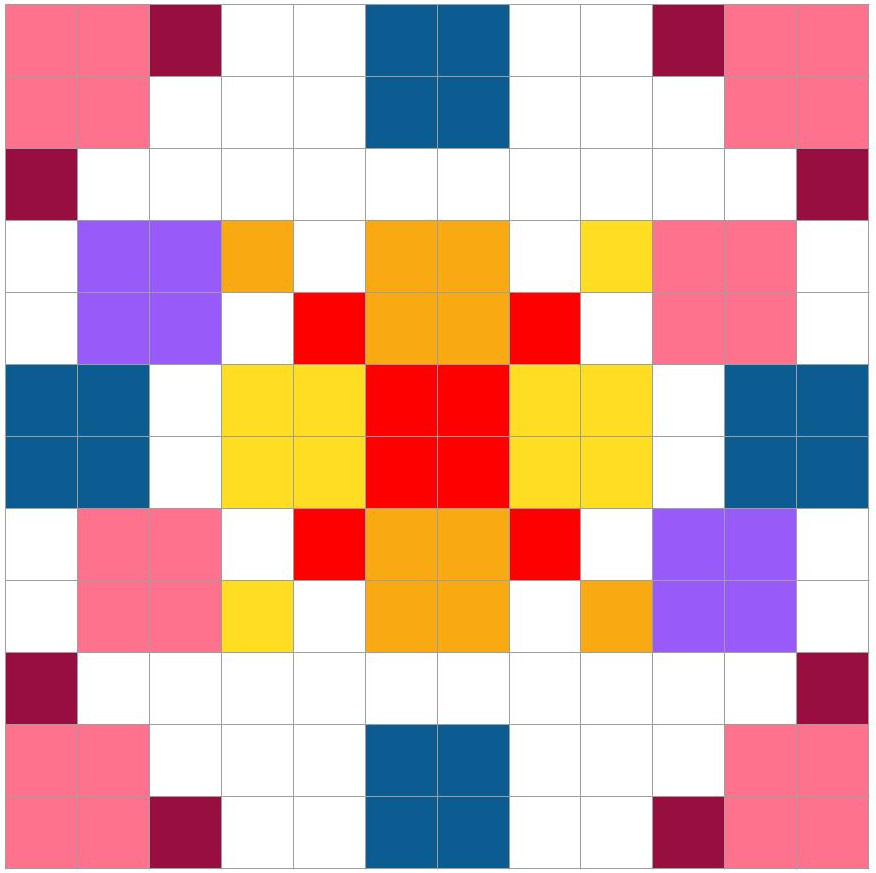
\includegraphics[scale=0.25]{First_ever.jpg}
\caption{Mosaic created with Beautiful Empathy}
\label{fig:mosaic}
\end{figure}

\lvl{Beautiful Empathy}

Beautiful Empathy is a collaborative board game in which players create a unique colored mosaic. The game has no scoring system and there is no official winner. The main outcome is the mosaic built together. Beautiful Empathy is conceived as a two player game, but the rules can be easily adapted to host more players. 

\vspace{1cm}
\lvl{Theme}

Lita loves art. She is happy when surrounded by beauty. For her house, Lita wants to build a large mosaic unlike any before. To produce a completely original piece, she hires her favourite artists (the players) and makes them work in turns on a shared mosaic. For the artists, it is important to work for people who understands them. Who can empathize with them. When Lita guesses their minds, artist are more productive and resourceful. By the end, all that matters is that the painters, and of course Lita, are happy with the resulting artpiece.
\newpage
\lvl{Game Script}

Beautiful Empathy is played in a series of consecutive paiting turns. On each turn, one player is the painter and another Lita. Typically the roles rotate normally among players, but alterations on who plays Lita are allowed. 

\vspace{1cm}
\lvl{The Empathy}

Each turn has two phases, the empathy and the beauty. In the first part, the empathy, Lita tries to figure out which word would the painter use to complete a sentence (out of two optional words). For example:

\begin{centering}
\texttt{Sentence:}\\
\textit{The tree was --------- in the middle of the forest}\\
\texttt{Options:}\\
\textit{shaking} | \textit{shinning}\\
\end{centering}
\vspace{0.5cm}

The painter must first read the sentence outloud with the two options, and quickly decide by instinct (and in silence) which one feels better. Lita must then guess which of the two options the painter chose. Empathy is key in this part.

Do a round of 5 questions, and count the number of correct ones. More correct answers by Lita will better motivate the painter for the second part of the turn, the beauty. 

During this part, and in this order, the painter:
\begin{itemize}
 \item tries to \textit{add a new color} to it's palette
 \item draws cards to \textit{see the shapes available}
 \item \textit{place the tiles} on the mosaic
\end{itemize}

The painter can use any combination of colors in its palette when placing the tiles. Once all tiles have been placed, the turn is over and a new one can begin.

\lvl{Add a New Color}

Each player starts the game with one color. Use a random generator between 1 and 20 for that, or choose freely if you prefer. This is about having fun.

\begin{figure*}[th!]
\centering
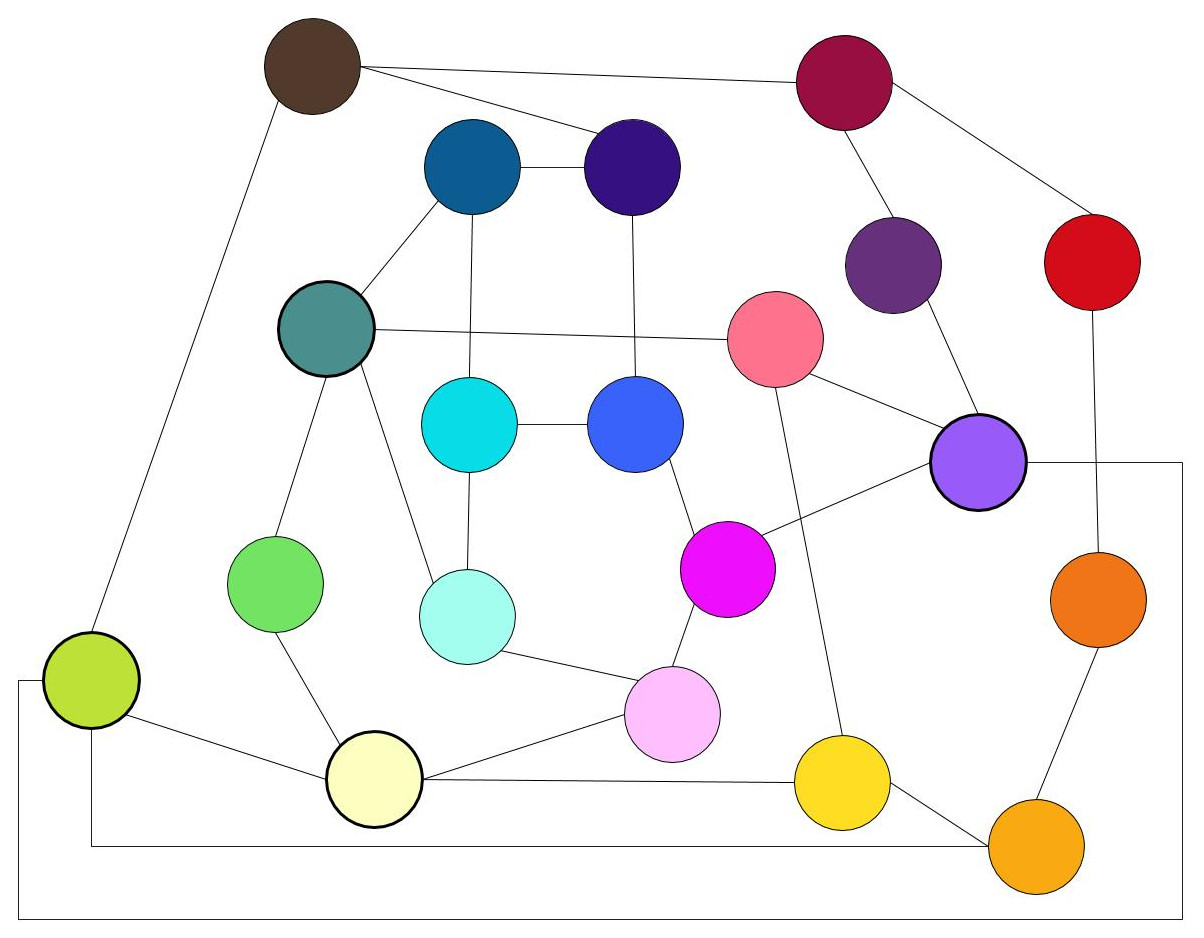
\includegraphics[scale=0.39]{color_map.jpg}
\caption{Color map. Edges between colors indicates direct connection, used to add them during the begining of the Beauty phase.}
\label{fig:color_map}
\end{figure*}

To gain a new color during your turn as a painter, first count the number of correct guesses from Lita. If the number of correct answers is bigger than the number of current colors in the painter pallette, the painter can add a new color to it. For example, a painter who owns 2 colors will get a new color if 3 or more questions were correctly answered by Lita. Five correct answers will always get the painter a new color, regardless of the colors already owned.

The painter can choose the color to gain among those directly connected in the color map with a color already owned. Mark the colors each player owns in the color map.


\lvl{See Available Shapes}

After trying to get a color, the painter will find the material it has to work on the mosaic. This will also depend on Litas empathy, as two or more correct guesses makes the painter highly motivated, while one or less correct guesses do not. Based on this, the painter draws a card from one of two decks. 
\begin{itemize}
    \item \textbf{Highly-Motivated}:
    \begin{itemize}
        \item 20\%: 8 small squares (1x1)
        \item 40\%: 4 small squares + 2 big squares (2x2)
        \item 30\%: 8 small squares + 2 big squares 
        \item 10\%: 16 small squares
    \end{itemize}
    \item \textbf{Any day}
    \begin{itemize}
        \item 70\%: 4 small squares
        \item 20\%: 4 small squares + 1 big square 
        \item 10\%: 8 small squares
    \end{itemize}
\end{itemize}


\lvl{Place the Tiles}

All that is left to do is for the painter to place the tiles on the mosaic. The painter has absolute freedom to do so, while the other painters can comment on the artistic aspects of it, before and after it is done. The placed tiles can be of any color available in the painter's pallette, and in any combination (different tiles, different colors).

\lvl{Inspiration Bonus}

If Lita got 5 correct answers, the painter gains a bonus action, moved by her empathy. The painter draws from a uniform distribution of:
\begin{itemize}
    \item Choose and gift any color from the board to a fellow painter. 
    \item Place 8 tiles on the mosaic with any colors of your choice (owned or not).
    \item Change the color of 4 tiles already on the board to any of your choice (owned or not).
\end{itemize}


At this turn, this painter's turn is over. Call the next one in!

\lvl{End of Game}

The Game ends when the painters agree the mosaic is done, or when a player cannot place its tiles because of lack of space on the mosaic. Once this is happens, take a look at the mosaic you created through empathy, and enjoy the beauty of your collaborative creation.

% \bibliographystyle{plain}
% \bibliography{references}
\end{document}
